%\documentclass[10pt,twocolumn,letterpaper]{article}
\documentclass[10pt,letterpaper]{article}

\usepackage{cvpr}
\usepackage{times}
\usepackage{epsfig}
\usepackage{graphicx}
\usepackage{algorithm}
\usepackage{algpseudocode}
\usepackage{amsmath}
\usepackage{amssymb}
\usepackage{subcaption}

\newlength\myindent
\setlength\myindent{2em}
\newcommand\bindent{%
  \begingroup
  \setlength{\itemindent}{\myindent}
  \addtolength{\algorithmicindent}{\myindent}
}
\newcommand\eindent{\endgroup}

\algdef{SE}[SUBALG]{Indent}{EndIndent}{}{\algorithmicend\ }%
\algtext*{Indent}
\algtext*{EndIndent}

% Include other packages here, before hyperref.

% If you comment hyperref and then uncomment it, you should delete
% egpaper.aux before re-running latex.  (Or just hit 'q' on the first latex
% run, let it finish, and you should be clear).
\usepackage[breaklinks=true,bookmarks=false]{hyperref}

\cvprfinalcopy % *** Uncomment this line for the final submission

\def\cvprPaperID{****} % *** Enter the CVPR Paper ID here
\def\httilde{\mbox{\tt\raisebox{-.5ex}{\symbol{126}}}}

% Pages are numbered in submission mode, and unnumbered in camera-ready
%\ifcvprfinal\pagestyle{empty}\fi
\setcounter{page}{1}
\begin{document}

%%%%%%%%% TITLE
\title{A Scalable Peer-to-Peer Network Infrastructure For Autonomous Distributed Communication Between Robots in an Austere Environment}

\author{Michael Hodges\\
Northeastern University\\
{\tt\small hodges.m@northeastern.edu}
\and 
Matthew Kuhn\\
Northeastern University\\
{\tt\small kuhn.ma@norhteastern.edu}
\and
Nadiia Ramthun\\
Northeastern University\\
{\tt\small ramthun.n@northeastern.edu}
\and
Alexander Stults\\
Northeastern University\\
{\tt\small stults.a@northeastern.edu}
% For a paper whose authors are all at the same institution,
% omit the following lines up until the closing ``}''.
% Additional authors and addresses can be added with ``\and'',
% just like the second author.
% To save space, use either the email address or home page, not both
}

\maketitle
%\thispagestyle{empty}

\section{Introduction}
In this project we propose a distributed system based upon robots exploring a planet such as mars. Robots will be sent to a planet where commands will be sent to the system from an agency, such as NASA, and the commands will be distributed to the appropriate robot. The system will have a simple goal of exploring the planet to collect data. In so doing, each robot will have a relative x and y coordinate that will determine it's position as well as a unique identifier. Since the planet has no infrastructure the robots will be holding all of their communication systems on house and must conserve power. For this reason, the range of transmission will be limited. The robots will keep track of who is in range of them in order to route messages. The robots will need to transmit messages amongst each other to execute commands and send responses. Since NASA will have limited access to the robots on the planet, when the robots are given a command the nodes will need to select a leader to distribute the command to the appropriate robot based on some heuristic.

Some Scenarios we propose to solve are as follows:
\begin{enumerate}
    \item [1.] Locating and dynamically updating robots within range. 
    \item [2.] Broadcasting messages to all robots on the planet.
    \item [3.] Selecting a coordinator on the planet.
    \item [4.] Consensus? not sure how consensus will fit in....
\end{enumerate}
%-------------------------------------------------------------------------
\section{Algorithms Overview}\label{Section:algs}
In this section we will review the algorithms that we chose to implement in the project. This section will be a review of the algorithms and not how they were implemented in the system. In so doing we will review algorithms with relation to leader election, consensus, peer-to-peer, and reliable multi-cast.

\subsection{Leader Election} \label{subsection:bully}
A leader election algorithm chooses a process to act in a specific way. In general, a leader election has a calling process that initializes the election and participants in the election. Each process is given a unique identifier and the process with the highest identifier participating in the election becomes the leader. These algorithms are measured by network bandwidth utilization and turnaround time.

We elect to utilize the bully algorithm as described in section 15.2 of Coulouris' Distributed Systems: Concepts and Design \cite{Coulouris5}. Some key assumptions are that communication between processes is reliable and each process knows which processes have higher identifiers with which it can communicate with. There are three messages used in this algorithm:
\begin{enumerate}
    \item [1.] election: sent to announce an election
    \item [2.] answer: sent to respond to an election message
    \item [3.] coordinator: sent to announce the identify of the newly elected process.
\end{enumerate}

The election is began when after enough timeouts a process realizes that the coordinator has failed. If a process knows it has the highest identifier number it can simply send a coordinator message to the remaining processes to elect itself. If the process does not have the highest identifier number known that is not crashed it will send an election message to all processes with a higher identifier number then itself. The process waits for an answer within some specified time, $T$. If no answers come in the process elects itself as the coordinator by sending a coordinator message. A process will wait for a maximum time of $T'$ before starting another election. During the election if a process receives a coordinator message it sets the elected variable to the coordinators identifier. If a process receives an election message it sends an answer message and begins its own election. When a new process is started it will start the election process and if it has the highest identifier it will become the coordinator despite the current coordinator still functioning. In the worst case this algorithm requires $0(N^2)$ messages.

\subsection{Consensus}
Consensus can be seen as a problem of agreement, where one, or more, processes proposes a value and all of the other processes need to agree upon what that value should be. Leader election can be seen as a form of consensus as everyone agrees upon a leader, or the ID of the leader. For any consensus algorithm we have the following requirements:

\begin{enumerate}
    \item [] Termination: every correct process will set its decision variable
    \item [] Agreement: the decision variable of every correct process is the same.
    \item [] Integrity: If all processes propose the same value, then all correct processes in the decided state have chosen that value.
\end{enumerate}

For our application we will assume a synchronous system and follow the algorithm as described in section 15.5.2 of Coulouris' Distributed Systems: Concepts and Design \cite{Coulouris5}. The algorithm is grounded in basic multicast and assumes that up to $f$ of $N$ processes exhibit crash failures. The algorithm can be implemented as follows:

\begin{algorithm}
\caption{Algorithm for process $p_i \in g$; algorithm proceeds in $f+1$ rounds  }\label{alg:cap}
\begin{algorithmic}
\State $Values_i^1 \gets \{v_i\}$
\State $Values_i^0 \gets \{\}$
\For{$r$ in $1:f+1$}
    \State B-multicast($g$, $Values_i^r - Values_i^{r-1}$) \Comment{Send only values that have not been sent}
    \State $Values_i^{r+1} \gets Values_i^r$
    \While{in round $r$}
        \State On B-deliver($V_j$) from some $p_j$
            $Values_i^{r+1} \gets Values_i^{r+1} \cup V_j$
    \EndWhile
\EndFor
\State $d_i = minimum(Values_i^{f+1})$
\end{algorithmic}
\end{algorithm}

The algorithm first has processes collect proposed values from other processes. The algorithm loops for $f+1$ rounds in which each of the correct processes B-multicast the values between themselves. In the algorithm the variable $Values_i^r$ contains the set of proposed values known to process $p_i$ at the start of round $r$. Each process multicasts the set of values that it did not send in the previous round and then receives multicasts from other processes to update the list of new values. Since the process is synchronous there is timeout that is applied to each round. On termination the processes decide on the minimum value it received. Given we can have up to $f$ crashes we will still reach a value since the loop lasts for $f+1$ rounds.


\subsection{Peer-to-Peer}\label{subsection:peer2peer}
For the peer-to-peer overlay network we generally utilized Gnutella v0.4 \cite{gnutella4}. This version is associated with distributed search and provides functionality to handle this search however we will limit our discussion to that used in the project. The benefits of Gnutella v0.4 is that it is fault-tolerant to failure even if a multitude of peers go offline.

The exchange of information as well as registering system is done through a variety of descriptors that live inside of a message passed on the network. The commands utilized in this project are as follows: ping and pong.
\begin{enumerate}
    \item [] Ping: The ping command is used to discover hosts on the network. In so doing, a peer will broadcast a ping message and wait for responses, or pongs. The ping message contains no payload and is simply used to trigger a response from peers.
    \item [] Pong: The pong command is used to respond to ping commands. The pong message contains the port and IP address upon which the responding host can accept incoming connections. 
\end{enumerate}

In the official Gnutella v0.4 description there are other descriptors that can be used with the main ones being Query, QueryHits, and Push. However, this is generally of more use for finding specific files within a peer and thus does not apply to our system.


\subsection{Reliable Multicast}
Reliable multicast is simply multicast with a guarantee that all processes in the group must receive a message if any process receives that message. We can implement reliable multicast by simply using a basic multicast with a rebroadcast functionality. It should be noted that it does not matter if the original sending process gets the message to all the processes just that some process gets the message to the process. An algorithm for reliable multicast from \cite{Coulouris5} is as follows:

\begin{algorithm}
\caption{Reliable Multicast Algorithm}\label{alg:multicast}
\begin{algorithmic}
\State On initialization
\Indent
    \State $Received \gets \{\}$
\EndIndent

\State For process $p$ to R-multicast message $m$ to group $g$
\Indent
\State $B-multicast(g,m)$ \Comment{$p \in g$ is included as a destination}
\EndIndent
\State On B-deliver($m$) at process $q$ with $g$ = group($m$)
\Indent
\If{ $m \notin Received$}
    \State $Received \gets Received \cup \{m\}$
    \State if( $q \neq p$) then B-multicast($g$, $m$); end if
    \State R-deliver m;
\EndIf
\EndIndent
\end{algorithmic}
\end{algorithm}

As can be seen a process starts with an empty buffer called received. If the process receives a message that it has not yet seen it adds it to the buffer and then multicasts it to the group. It should also be noted that when a process multicasts it sends to itself and therefore it performs a check to ensure it does not continuously multicast.


%-------------------------------------------------------------------------  
\section{Implementation Details}
In this section we will outline how the algorithms presented in section \ref{Section:algs} were implemented in our project and the necessary modifications that were made.
\subsection{Controller}
The Controller package is responsible for handling the main communications between the robots, which are represented as Peer objects.
    \subsubsection{Message Routers}
    MessageRouters are used to route MessageChannels to the Peer, and to enable the Peer to make decisions about what to do with messages once they have been received. The router takes in a channel and uses its identifier to determine which MessageRoute to use send it to the Peer. It then generates a MessgeEvent, which is sent to the Peer's MessageListener, and from there the Peer can decide what to do with the message.
    \subsubsection{Message Routes}
    MessageRouters contain a collection of MessageRoutes, which have different identifiers for different functions of the Peers. The only other attribute that a message route has is its MessageListenerFactory, which is passed in from the Peer which creates the Route. This MessageListenerFactory is used to create new MessageListeners whenever a MessageChannel is received, to generate events for the Peer to act on. 
    \subsubsection{Message Channels}
    A MessageChannel is the method for Peers to receive incoming messages, and to create messages to send to other Peers. They take in a TCP Socket connection, and use that to write incoming messages to a buffer, which the receiving Peer will be able to read out.  
    \subsubsection{TCP}
    The TCP package provides the TCPServer which Peers will use to to receive incoming communications. The server will run on a Thread in the background, and creates MessageChannels using incoming sockets, and then routes them to the Peer using a MessageRouter passed in by the Peer.
\subsection{Overlay Network}
The overlay network is responsible for locating in range robots. This package consists of two classes called shortwave radio and broadcast listener. The shortwave radio class implements the ping algorithm and also has a broadcast listener object that listens for periodic multicast messages to respond (pong) to.
    \subsubsection{ShortwaveRadio}
    This class is used to periodically send a ping to the multicast group of robots. In Gnutella v0.4 a peer only sends a ping once it originally joins the group, but since our robots are moving about the number of nodes in range will change. In so doing, the shortwave radio broadcasts a ping every 3 seconds and will update a hashmap of the ID and port number of robots within range. All robots that do not respond within a specified timeout will be dropped from the hashmap. Therefore, our method is robust to failures because the robots that can be reached will be periodically updated maintaining an accurate list. Furthermore, if a robot goes offline and comes back online it will be added back in without any issues. Since we are actively updating the list we utilize UDP packets to send the message and if a packet gets dropped it will most likely be sent successfully in the future.
    \subsection{BroadcastListener}
    This class listens on a specified port for multicast messages. When a message comes in that is specified as "ping" the class will respond with a "pong" message that specifies it's local ID and the port with which it can receive incoming messages. Since we do not have an actual deployment of robots the broadcast listener will receive every single ping message. To simulate being out of range we set a max range and do a check inside this class. If the distance between the sending and receiving node is within the max range then a pong is returned, if not no message is sent.
\subsection{Model}
    The model package of the code base contains the interfaces and implementations for the Peer objects, along with the wrapper functionality for the bully algorithm, and the client code to run the various simulation scenarios using the Peer objects.
    \subsubsection{Bully} 
    The bully package contains the interface and implementation of BullyParticipant nodes, which are created and used by Peer nodes as proxy objects to participate in the bully algorithm of leader election. These BullyParticipant objects use the same host address and port numbers as the Peers which own them, and serve as an abstraction of the BullyAlgorithm functionality, in order to simplify the Peer interface. The BullyAlgorithm class implements the logic of the bully algorithm, as described in section \ref{subsection:bully}. The Peer accepts communications related to the bully algorithm using its TCPServer object, and then passes along the commands to the BullyParticipant object which exists within the scope of each Peer object. 
    \subsubsection{Simulation}
    The sim package of the model contains the implementation of the Simulation class, as well as the ChaosClient class. The ChaosClient takes advantage of the ChaosMessageRoute from the controller to expose functionality to block or unblock a certain message route in the ChaosMessageRouter. This can be used to simulate a loss of connection between Peers. The simulation provides various scenarios in which the Peers can demonstrate the different functionalities of distributed systems, as described below in the Experiments section.
    \subsubsection{Consensus}
    The architecture of the Consensus algorithm is similar to the BullyAlgorithm, in that it provides a ConsensusParticipant interface for the Peer to use to create a proxy version of itself to use to participate in the Consensus algorithm. This abstracts the Consensus functionality away from the Peer, into its own package. The consensus algorithm is used by the Peers to maintain a consensus on which nodes are available to the network. When a Peer becomes the leader of the Bully Election, it will start a consensus vote to determine who is currently in range of the ShortwaveRadio. The consensus package uses a ConsensusListenerFactory object to handle Consensus ActionEvents passed to it by the ConsensusParticipant object within a Peer. This is triggered by the same mechanism in the MessageRouter as is triggered by all other users of the MessageRouter control infrastructure.
    \subsubsection{Peer}
    The Peer is the main object model representation of the "robots" on mars. The Peer has a port number and hostname (localhost) that it uses to receive communications from other peers, and it shares this hostname and port number with its instance of a BullyParticipant. The Peer also uses a ShortWaveRadio, with the same hostname and a port number 1000 higher that its standard port, which is used in the Overlay Network to find in-range Peers to communicate with. The Peer has a MessgeRouter which it uses in conjunction with the TCPServer to receive and properly route messages. It also uses a MessageChannelFactory to create new MessageChannels to execute outward communication to other Peers. The PeerClient class uses external programmatic access to the Peer interface to enable the main Program to create Peers and tell them what to do.
    
    The Peer object class also implements the reliable multicast. When implementing reliable multicast we will need to use FIFO ordering with multicast, in order to ensure that all messages and commands from the leader to the rest of the robots are received in the proper execution order. Within this system, order of message receipt by the robots is crucial, as executing commands out of order could have disastrous consequences, including the loss of a robot. Our multicast system will maintain reliability by ensuring integrity, validity, and agreement. To ensure the system's integrity, we will ensure that a process only delivers each message at most one time. The way that this is checked is to include a unique message identifier on each multicast message. Upon receiving a message, a robot will check the message ID, and only proceeds with executing that request and forwarding it to all other members if it has not already seen the message. For validity, we must ensure that if process multicasts a message, then that message will eventually be delivered. Finally, to guarantee agreement, we will ensure that if one process delivers a message, then all other members of the group will also eventually deliver that message.
    
    \subsubsection{Coordinator}
    The Coordinator serves the role of NASA in our scenarios, in that it assists the robots in establishing contact with one another. The Coordinator exposes registerNode and getNodes functionality, so whenever a new robot turns itself on, it contacts the Coordinator (NASA) to register itself, and to receive a list of other robots which have already turned themselves on and registered with the coordinator. Once the robot receives this list, the Peer uses its own communications functionality to reach out to the previously established Peers, and notify those Peers of its own existence.
    
    Whenever a robot receives a multicast message, it will log the ID of the message, and then execute the command. Once this has happened, the robot will multicast the message to all of its peers, in case one of them had not yet received the message. If a robot receives a message and it has an ID that the robot has already seen, it does not execute the message again, and does not forward it on to the peers, since it will have already taken both of those actions the first time it saw that message. 
    
\subsection{View}
The view package provides a method for visualizing robots, and showing how they perceive their relationships with the other relationships in the environment. It also will display the changing status of robots as the simulations are run, to display the efficacy of our algorithms.        
        \begin{figure}[!t]
            \centering
            \begin{subfigure}{0.475\textwidth}
                \centering
                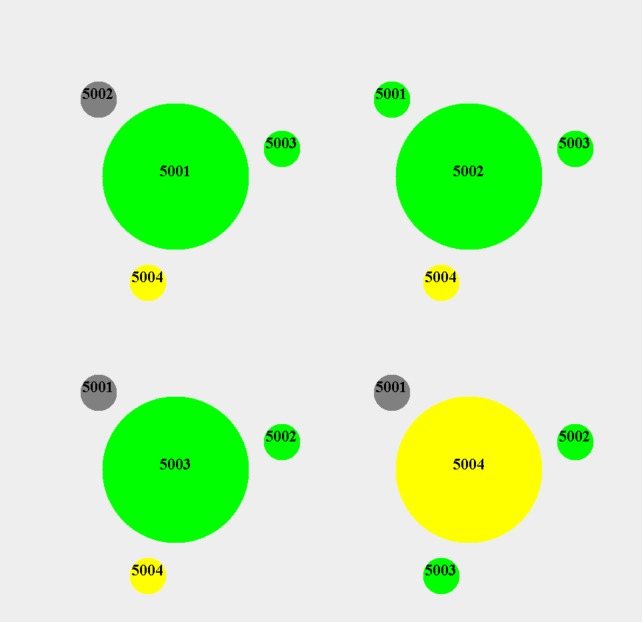
\includegraphics[width=\textwidth]{images/peers_and_leader.jpeg}
                \caption{Node 5002 out of range}
                \label{img:subA}
            \end{subfigure}
            \begin{subfigure}{0.475\textwidth}
                \centering
                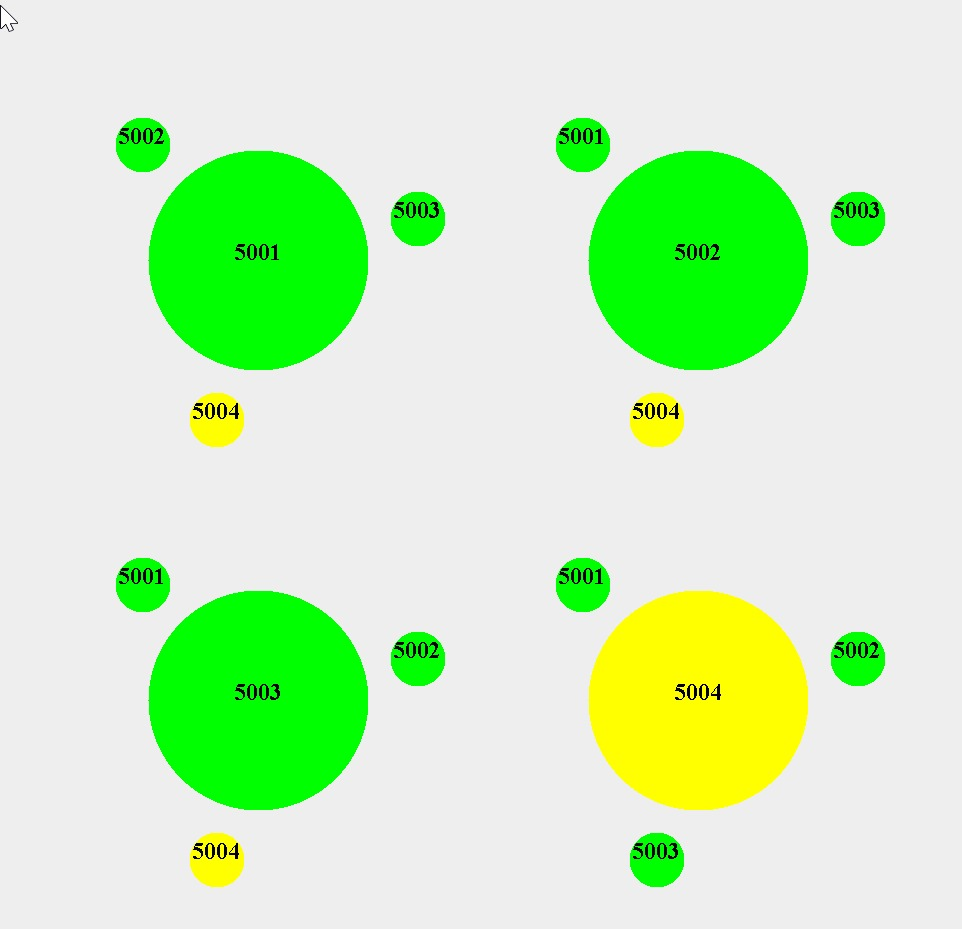
\includegraphics[width=\textwidth]{images/gohome.jpeg}
                \caption{Multicast go home}
                \label{img:subB}
            \end{subfigure}
            \begin{subfigure}{0.5\textwidth}
                \centering
                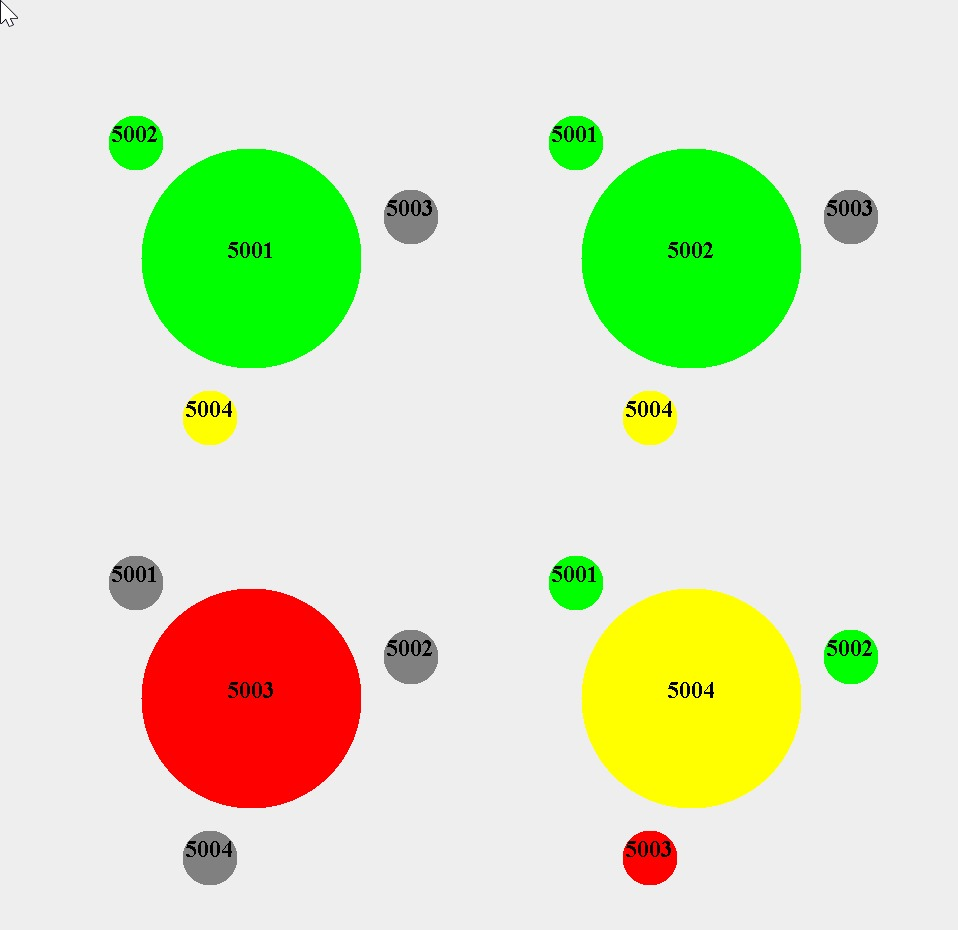
\includegraphics[width=\textwidth]{images/failure.jpeg}
                \caption{Node Failure}
                \label{img:subC}
            \end{subfigure}
                \caption{Peers status. Green: up, Yellow: Leader, Grey: unknown}
                \label{img:peers_and_leader}
        \end{figure}
    \subsubsection{Entity/Robot}
    The first key element of the GUI package is the combination of the Robot and Entity interfaces. These two interfaces are the visual representation of the Peer objects, and provide an interface for both displaying and changing the graphical properties of the display. The Robot is wrapped by the RemoteRobot interface, which extends Remote functionality, to enable the Robots to register themselves with the remote dashboard. The Robots are functionally separated from the Peer objects by ActionListeners. The key to making this happen is the PeerEventHandler class. This class is initialized with a Peer object, and is passed to that Peer object as an ActionListener. Whenever the status of a Peer object changes in any meaningful way, it will emit an event to the ActionListener, which will process the event and update the appropriate Robot object.
    \subsubsection{Dashboard}
    The second major element of the GUI package is the Dashboard. This is the main centerpiece of the graphical display, which, among other things, is a JPanel. The dashboard allows entities to be registered with it, and it will then paint itself with those entities. It keeps track of the various entities by storing them in a World object, which allows for access to entities, and has a size which is used to determine display size. The Dashboard is wrapped by the RemoteDashboard, which adds Java Remote functionality, allowing for entities to register themselves with the dashboard server over a port, instead of needing to exist as local objects. This is in line with the rest of the project architecture, where the Peers themselves each run as their own Java process.

    
%------------------------------------------------------------------------

\section{Experiments}
In this section we will outline some scenarios that were played out to showcase our project. A simulation GUI was created to show a group of nodes with communication statuses and leader status. 
        

\subsection{Node Failure}
Looking at the set of figures in figure \ref{img:peers_and_leader} we can see a group of nodes with process ID's 5001 to 5004. The processes are located with the ping-pong messaging outlined in section \ref{subsection:peer2peer} and it should be noted that each process has located and communicated with one another initially. As can be seen the process 5002 has suffered some sort of error and is no longer communicating and thus is greyed out while the remaining processes, yellow and green, are still communicating.

\subsection{Reliable Multicast}
The operation of multicast can be seen in figure \ref{img:subA} and \ref{img:subB}. In this figure we see that multiple nodes are out of range. A command is issued to all nodes to "Go Home" and the result can be seen in figure \ref{img:subB} where now all of the nodes are in range of each other.

\subsection{Bully Election}
When the processes establish initial communication a bully leader election is called. This election is done as is outlined in section \ref{subsection:bully}. As can be seen in figure \ref{img:peers_and_leader} the process with the highest ID, 5004, was selected and is colored yellow. We can see that each node agrees that 5004 is the leader as each set of nodes has process 5004 colored yellow to denote that it is the leader. When process 5004 fails a new election is started and the next highest process is elected, 5003. This is visualized in figure .

\subsection{Consensus}
The consensus algorithm is started from the elected leader in and is used to keep track of all of the available robots. In so doing, the leader asks all of the individual robots what robots they can see. If a majority see a specific robot then the leader concludes that the node is available if a majority cannot see a robot the leader concludes the node has failed. These failures can be seen in figure \ref{img:subC}.
%------------------------------------------------------------------------
\section{Conclusion}
    Accomplishing the task of creating any sort of distributed system in which the various nodes have imperfect information about their peer nodes presents with multiple problems. The nodes must be able to perform tasks concurrently, especially in the case of robots traversing the Martian landscape. If only one robot could move at a time, no useful work would be able to be accomplished. Additionally, requiring one central communications server to relay all commands on a rolling basis introduces a single point of failure into the system. Our system's peer-to-peer nature, along with the reliable multicast functionality, removes this single point of communications failure, and allows the robots to continue executing their own tasks without waiting for a central server to reply to them. The consensus building and leader election functionalities allow for the robots to come to agreements about actions to take, again without the need for some pre-determined central authority which would introduce a single point of failure. These four methodologies working together form a system which is both fault-tolerant in its decision making, and robust in its communications methods, a perfect candidate for operation in the hostile terrain of another planet.
%Autofill citations while in insert mode do ctl-x, ctl-o
{\small
\bibliographystyle{ieee_fullname}
\bibliography{egbib}
}

\end{document}
